\documentclass[12pt,a4paper]{article}

\usepackage[a4paper,margin=1in]{geometry}
\usepackage{graphicx}
\usepackage{array}
\usepackage{float}
\usepackage{setspace}
\usepackage{longtable}
\usepackage[hidelinks]{hyperref}
\usepackage{caption}
\usepackage{needspace}

\setstretch{1.15}
\graphicspath{{./}{ResultImage/}{Logo/}}
\newcommand{\sectionbreakguard}{\Needspace{8\baselineskip}}
\newcommand{\subsectionbreakguard}{\Needspace{5\baselineskip}}

\begin{document}

\begin{titlepage}
\centering

\begin{minipage}{0.45\textwidth}
    \raggedright
    
\includegraphics[width=3cm]{ITC_Tran_Logo.png}
\end{minipage}
\begin{minipage}{0.45\textwidth}
    \raggedleft
    
\includegraphics[width=3cm]{AMS-Logo.jpg}
\end{minipage}

\vspace{1.5cm}

{\Large\bfseries INSTITUTE OF TECHNOLOGY OF CAMBODIA\par}

\vspace{0.4cm}

{\large\bfseries Department of Applied Mathematics and Statistics\par}

\vspace{1.8cm}

{\Large\bfseries Introduction to Parallel and Distributed Systems\par}

\vspace{0.4cm}

{\large I4-AMS-DAS-A (2025--2026)\par}

\vspace{1.8cm}

{\Large\bfseries RPC Project Report - BG Bank\par}

\vspace{2.4cm}

{\large Team 3 \par}
\begin{center}
\begin{tabular}{|p{6cm}|p{3.5cm}|p{2cm}|}
\hline
\textbf{Name of student} &
\textbf{ID of student} &
\textbf{Score} \\
\hline
1. KONG SATTHA & e20220963 & \dots \\
2. HENG MENGHONG & e20220258 & \dots \\
3. LY CHUNGHEANG & e20220980 & \dots \\
4. HEANG SOTHEARA & e20221213 & \dots \\
5. HEAM VISAL & e20221349 & \dots \\
\hline
\end{tabular}
\end{center}

\vfill

\begin{minipage}{0.6\textwidth}
\textbf{Lecturer:} Mr. KHEM Thay\\
\hspace*{1.8cm} Mr. KHEM Thay
\end{minipage}
\begin{minipage}{0.35\textwidth}
\raggedleft
(Course)\\
(TP)
\end{minipage}

\end{titlepage}

\tableofcontents
\newpage

\sectionbreakguard
\section{Abstract}

BG Bank is a secure banking web application built as a class project for Introduction to Parallel and Distributed Systems. The system demonstrates how a web client can communicate with separated backend services through Remote Procedure Call (RPC). The application uses Flask for the web interface, XML-RPC for distributed service communication, SQLite for storage, Fernet encrypted login tickets for session identity, hashed passwords for authentication, and a rule-based fraud detection module for transaction monitoring.

The main distributed design separates the application into a web layer, an authentication RPC service, a banking RPC service, and a database layer. This separation makes the project suitable for studying service boundaries, remote method calls, shared data access, and transaction workflows.

\sectionbreakguard
\section{Project Objectives}

The project objectives are summarized in Table~\ref{tab:project-objectives}.

\begin{longtable}{|p{1.2cm}|p{12.8cm}|}
\caption{Project objectives}\label{tab:project-objectives}\\
\hline
\textbf{No.} & \textbf{Objective} \\
\hline
1 & Build a banking web application with registration, login, profile, account, transaction, and fraud report features. \\
\hline
2 & Apply XML-RPC as a distributed communication mechanism between the web application and backend services. \\
\hline
3 & Protect login sessions using encrypted tickets and protect sensitive transactions using an action password. \\
\hline
4 & Store users, customer profiles, accounts, transactions, and audit logs in a database. \\
\hline
5 & Detect suspicious transaction behavior using rule-based fraud scoring. \\
\hline
6 & Run the system in a containerized environment using Docker. \\
\hline
\end{longtable}

\sectionbreakguard
\section{System Architecture}

The system is divided into independent components. The browser communicates with the Flask web application. The Flask application does not directly perform all authentication and banking work; instead, it calls XML-RPC services. The authentication service handles registration and login, while the banking service handles balance, deposit, withdraw, transfer, history, profile, audit log, and fraud report operations. SQLite stores all persistent application data.

\begin{figure}[H]
    \centering
    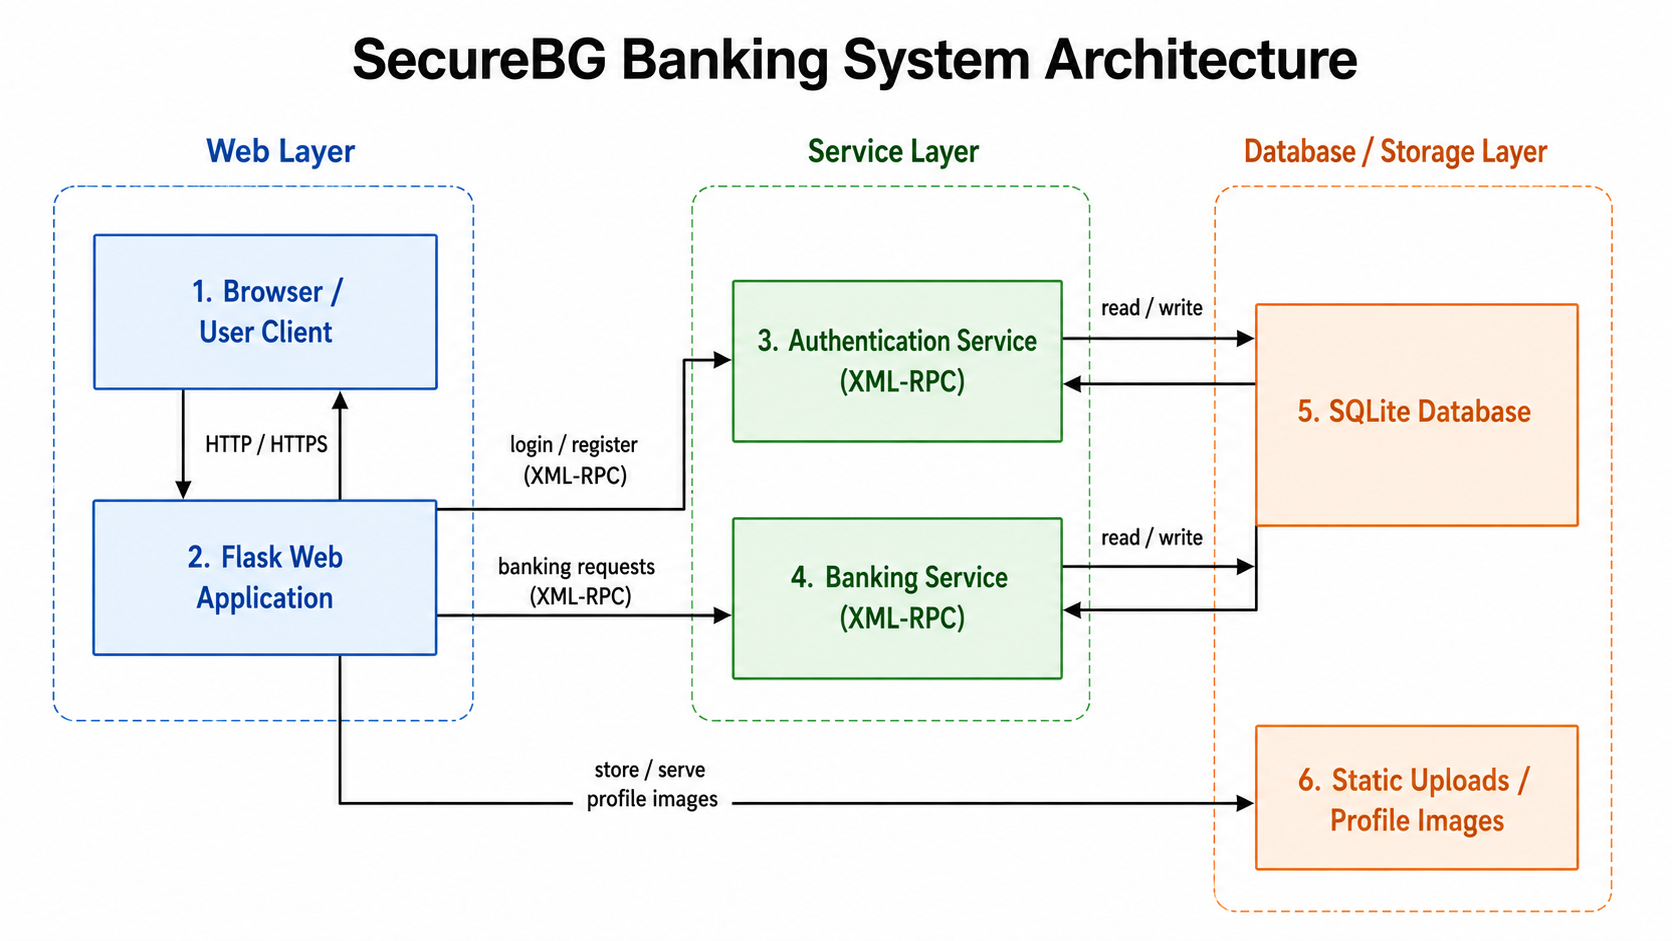
\includegraphics[width=\textwidth]{System-Architecture-Diagram-GPT.png}
    \caption{SecureBG banking system architecture}
\end{figure}

\subsectionbreakguard
\subsection{Main Components}

\begin{longtable}{|p{4cm}|p{10cm}|}
\hline
\textbf{Component} & \textbf{Responsibility} \\
\hline
Browser & Provides the user interface for registration, login, dashboard, profile, transactions, and fraud report pages. \\
\hline
Flask Web App & Handles routes, forms, sessions, page rendering, and RPC calls to backend services. \\
\hline
Authentication RPC Service & Validates registration and login requests, hashes passwords, creates user records, and issues encrypted login tickets. \\
\hline
Banking RPC Service & Validates tickets, loads accounts, processes deposits, withdrawals, transfers, histories, profiles, and fraud reports. \\
\hline
Fraud Detection Module & Applies transaction risk rules and returns a risk score, fraud flag, and reasons. \\
\hline
SQLite Database & Stores users, profiles, accounts, transactions, and audit logs. \\
\hline
Docker & Provides a repeatable runtime environment for the web and RPC services. \\
\hline
\end{longtable}


\subsectionbreakguard
\subsection{Detailed Component Description}

This project is organized as a distributed application with clear service responsibilities. Each component has a separate role, but all components work together to complete the banking workflow.

\subsubsection{Client Browser}

The client browser is the user-facing part of the system. It displays the web pages for registration, login, dashboard, deposit, withdraw, transfer, transaction history, fraud report, profile, and about page. The browser does not communicate directly with the authentication service, banking service, or database. It only sends HTTP requests to the Flask web application.

\subsubsection{Flask Web Application}

The Flask web application is the presentation and coordination layer. It receives form submissions from the browser, validates basic input, manages the user session, renders HTML templates, stores the encrypted login ticket in the session, and sends XML-RPC requests to the backend services. For example, when a user deposits money, Flask receives the amount from the deposit form and calls the banking RPC service with the login ticket and deposit amount.

\subsubsection{Authentication RPC Service}

The authentication RPC service is responsible for identity management. It handles user registration and login. During registration, it checks required fields, hashes the login password and action password, creates the user record, creates the customer profile, creates the bank account, and writes an audit log. During login, it verifies the submitted password and returns a Fernet encrypted ticket. This ticket contains the username, issue time, and expiry time.

\subsubsection{Banking RPC Service}

The banking RPC service is responsible for protected banking operations. Every banking request must include a valid encrypted ticket. The service decrypts the ticket, identifies the current user, checks account status, and then performs the requested operation. Deposit requires only a valid ticket, while withdraw and transfer also require the action password. The banking service also loads dashboard data, transaction history, fraud reports, profile information, and audit logs.

\subsubsection{Security Module}

The security module provides reusable security functions for the web application and RPC services. It creates and loads the Fernet key, encrypts and decrypts login tickets, checks ticket expiry, hashes passwords, verifies passwords, and derives a stable Flask secret key. This module allows the authentication service and banking service to share the same ticket validation logic.

\subsubsection{Fraud Detection Module}

The fraud detection module checks transaction behavior using fixed rules. It calculates a risk score based on account status, large transaction amount, unusual amount compared with the average transaction amount, many transactions in a short time, large balance drop, many transfer receivers, and daily transfer limit. The output includes a fraud flag, risk score, and explanation reasons. These results are stored with the transaction record and shown in the fraud report page.

\subsubsection{SQLite Database}

The SQLite database stores all persistent data for the system. It contains users, customer profiles, accounts, transactions, and audit logs. The authentication service and banking service access the same database through helper functions in the database module. This makes the database a shared storage layer for both RPC services.

\subsubsection{Docker Environment}

Docker and Docker Compose provide a repeatable environment for running the system. The deployment starts the Flask web application, authentication RPC service, and banking RPC service as separate services. This supports the distributed-system goal of the project because each service can run as an independent process while communicating through RPC.

\subsectionbreakguard
\subsection{Component Interaction Summary}

\begin{longtable}{|p{4cm}|p{10cm}|}
\hline
\textbf{Interaction} & \textbf{Description} \\
\hline
Browser to Flask & The user submits forms and views rendered pages through normal HTTP requests and responses. \\
\hline
Flask to Authentication RPC & Flask sends registration and login requests to the authentication service through XML-RPC. \\
\hline
Flask to Banking RPC & Flask sends banking requests such as deposit, withdraw, transfer, history, profile, and fraud report requests through XML-RPC. \\
\hline
Authentication RPC to Database & The authentication service writes user, profile, account, and login audit data into SQLite. \\
\hline
Banking RPC to Database & The banking service reads and updates account balances, transactions, profiles, fraud data, and audit logs. \\
\hline
Banking RPC to Fraud Detection & The banking service calls the fraud detection module before recording deposit, withdraw, and transfer transactions. \\
\hline
Security Module to Services & The authentication service uses the security module to create tickets, while the banking service uses it to validate tickets. \\
\hline
\end{longtable}

\sectionbreakguard
\section{Technologies Used}

\begin{longtable}{|p{4cm}|p{10cm}|}
\hline
\textbf{Technology} & \textbf{Use in the project} \\
\hline
Python & Main programming language for the web application, RPC services, database layer, fraud detection, and security helpers. \\
\hline
Flask & Web framework for routes, sessions, form handling, and HTML template rendering. \\
\hline
XML-RPC & Communication protocol used by Flask to call authentication and banking service methods. \\
\hline
SQLite & Local database for persistent users, profiles, accounts, transactions, and audit logs. \\
\hline
Fernet encryption & Symmetric encryption mechanism used to create protected login tickets. \\
\hline
Password hashing & Mechanism used to store login passwords and action passwords without saving plain text secrets. \\
\hline
Docker and Docker Compose & Container tools used to run the web application and RPC services in a repeatable environment. \\
\hline
HTML, CSS, and JavaScript & Frontend technologies used to build the browser interface. \\
\hline
\end{longtable}

\sectionbreakguard
\section{RPC Service Design}

The project uses XML-RPC to separate the browser-facing web application from the backend service logic. Instead of placing all business logic inside Flask routes, the web application calls remote methods exposed by two backend services. This design supports the distributed-system objective of the project because authentication and banking operations run as separate processes with clear interfaces.

Each RPC method returns a structured response containing a success value, a message, and optional data. This makes the communication predictable for the Flask web layer. Flask can call a remote method, check whether the operation succeeded, display the response message to the user, and render the returned data in the correct page.

\subsectionbreakguard
\subsection{Authentication Service}

The authentication service exposes the identity-related methods of the system. It is responsible for registration and login, so the Flask web application does not directly create login tickets or verify password hashes.

\begingroup
\small
\setlength{\tabcolsep}{4pt}
\begin{longtable}{|p{5.7cm}|p{8.3cm}|}
\hline
\textbf{RPC Method} & \textbf{Purpose} \\
\hline
\texttt{register\_user}\newline\texttt{(registration\_data)} & Receives registration and profile data from Flask, validates required fields, normalizes the username, hashes the login password and action password, creates the user record, creates the customer profile, creates the bank account, and records a registration audit log. \\
\hline
\texttt{login(username, password)} & Receives login credentials from Flask, normalizes the username, loads the user record, verifies the submitted password against the stored password hash, updates the last login time, writes a login audit log, and returns an encrypted login ticket when authentication succeeds. \\
\hline
\end{longtable}
\endgroup

The authentication service is important because it is the only component that issues login tickets. After login succeeds, the ticket becomes the proof of identity used by the banking service. This avoids sending the login password repeatedly for every banking operation.

\subsectionbreakguard
\subsection{Banking Service}

The banking service exposes the account, transaction, profile, dashboard, audit, and fraud-report operations. Every method that handles customer data receives the encrypted login ticket from Flask. The service validates the ticket before reading or changing account data.

\Needspace{10\baselineskip}
\begingroup
\small
\setlength{\tabcolsep}{4pt}
\begin{longtable}{|p{5.7cm}|p{8.3cm}|}
\hline
\textbf{RPC Method} & \textbf{Purpose} \\
\hline
\texttt{get\_balance(ticket)} & Validates the login ticket and returns the current account balance and currency. \\
\hline
\texttt{deposit(ticket, amount)} & Validates the ticket and amount, loads the account, calculates the new balance, runs fraud detection, updates the balance, records the transaction, and writes an audit log. \\
\hline
\texttt{withdraw(ticket,}\newline\texttt{amount,}\newline\texttt{action\_password)} & Validates the ticket, amount, account status, action password, and available balance before updating the balance and saving the transaction. \\
\hline
\texttt{transfer(ticket,}\newline\texttt{receiver\_username,}\newline\texttt{amount,}\newline\texttt{action\_password)} & Validates the sender ticket, receiver, amount, action password, sender balance, and receiver account status. It then updates both balances, records outgoing and incoming transaction rows, and writes audit logs for both users. \\
\hline
\texttt{view\_transaction}\newline\texttt{\_history(ticket)} & Returns all transaction records for the authenticated user. \\
\hline
\texttt{detect\_fraud(ticket)} & Calculates the current user risk report by loading suspicious transactions and summarizing risk reasons. \\
\hline
\texttt{trust\_fraud}\newline\texttt{\_report(ticket)} & Allows the user to trust suspicious transaction results by resetting suspicious fraud flags and risk scores for their own transactions. \\
\hline
\texttt{get\_risk}\newline\texttt{\_score(ticket)} & Returns a compact risk score and reason list for dashboard use. \\
\hline
\texttt{get\_user}\newline\texttt{\_profile(ticket)} & Returns the authenticated user profile, account information, user role, user status, and last login time. \\
\hline
\texttt{update\_user}\newline\texttt{\_profile(ticket,}\newline\texttt{profile\_data)} & Validates editable profile fields and updates the customer profile. \\
\hline
\texttt{get\_account}\newline\texttt{\_details(ticket)} & Returns account number, account type, balance, currency, status, and limit data. \\
\hline
\texttt{get\_dashboard}\newline\texttt{\_summary(ticket)} & Combines profile, account, recent transactions, total transaction count, risk score, and last login data for the dashboard page. \\
\hline
\texttt{get\_audit}\newline\texttt{\_logs(ticket)} & Returns audit log records for the authenticated user. \\
\hline
\end{longtable}
\endgroup

\subsectionbreakguard
\subsection{RPC Response Format}

The services use a common response format:

\begin{verbatim}
{
    "success": true or false,
    "message": "Human-readable result message",
    "data": {... optional returned data ...}
}
\end{verbatim}

This response pattern simplifies communication between Flask and the RPC services. The web application does not need to understand internal service details. It only checks the success flag, shows the message, and uses the data field when rendering the dashboard, profile, transaction history, or fraud report.

\subsectionbreakguard
\subsection{Transfer Workflow}

Transfer is the most complete distributed workflow because it uses the web app, banking RPC service, security module, database, and fraud detection module.

\begin{figure}[H]
    \centering
    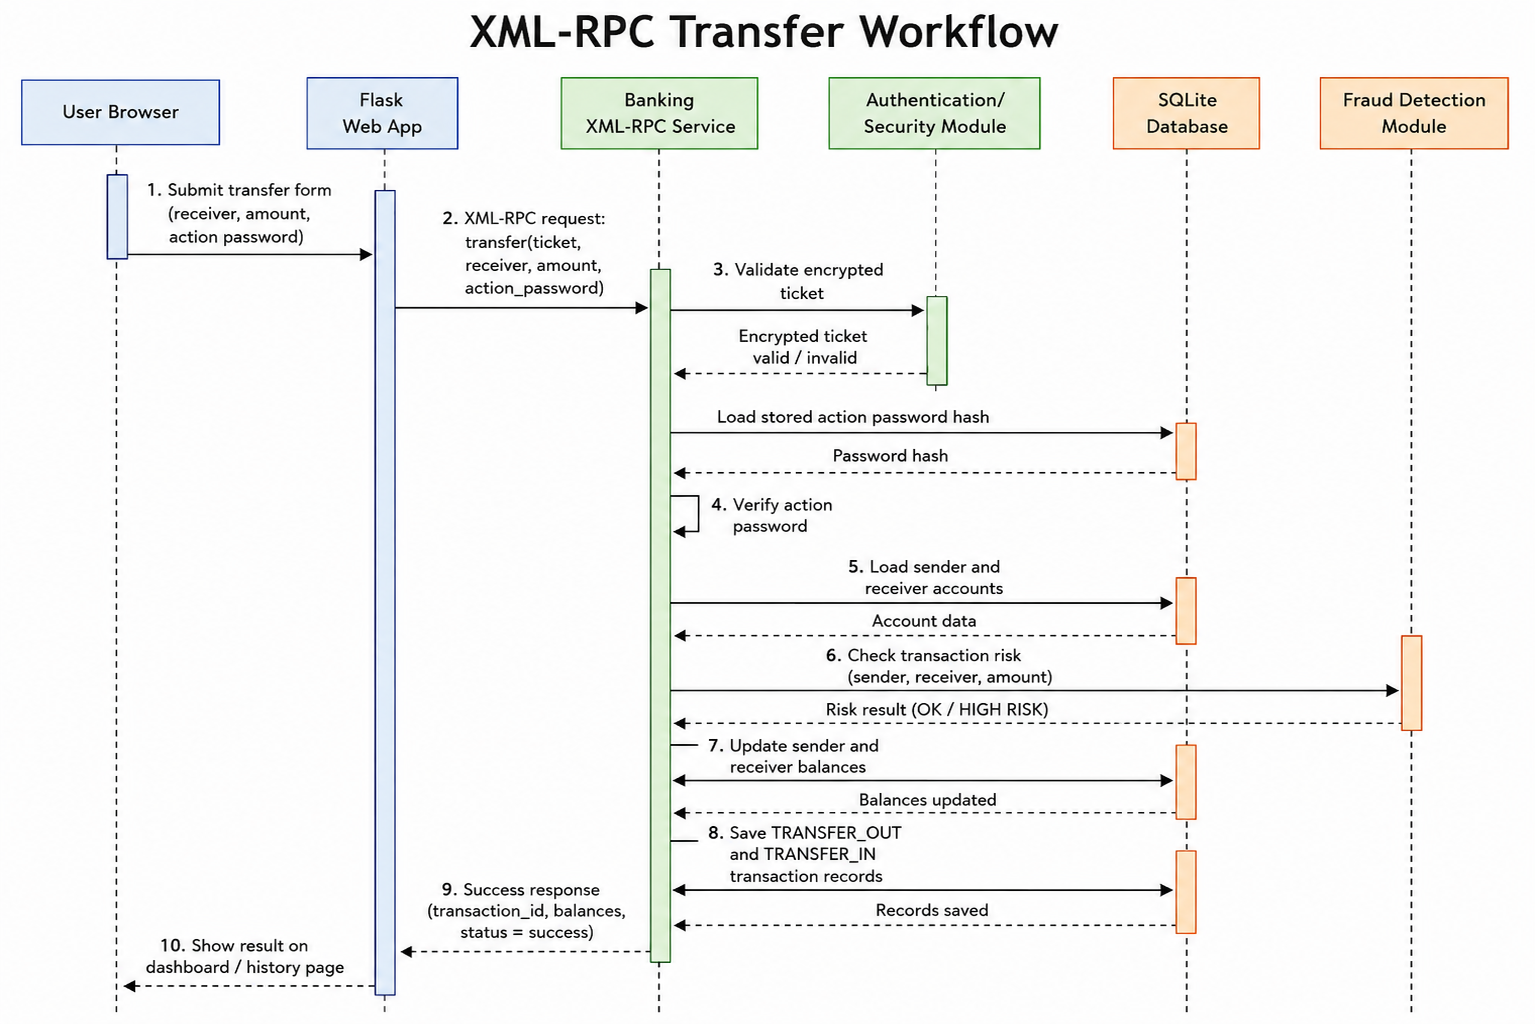
\includegraphics[width=\textwidth]{RPC-Workflow-Diagram-GPT.png}
    \caption{XML-RPC transfer workflow}
\end{figure}

The transfer workflow is summarized in Table~\ref{tab:transfer-workflow}.

\begin{longtable}{|p{1.2cm}|p{12.8cm}|}
\caption{Transfer workflow steps}\label{tab:transfer-workflow}\\
\hline
\textbf{Step} & \textbf{Description} \\
\hline
1 & The user submits receiver, amount, and action password in the Flask web app. \\
\hline
2 & Flask calls the banking XML-RPC method with the encrypted ticket and transfer data. \\
\hline
3 & The banking service decrypts the ticket and identifies the sender. \\
\hline
4 & The service validates the action password. \\
\hline
5 & Sender and receiver accounts are loaded from SQLite. \\
\hline
6 & The service checks balance and calculates new balances. \\
\hline
7 & Fraud detection checks transaction risk. \\
\hline
8 & Sender and receiver balances are updated. \\
\hline
9 & Transfer transaction records and audit logs are saved. \\
\hline
10 & The result is returned to Flask and displayed to the user. \\
\hline
\end{longtable}

\sectionbreakguard
\section{Database Design}

The database contains five main tables: users, customer profiles, accounts, transactions, and audit logs. The project uses logical relationships between these tables through fields such as username and account number. The schema diagram shows these logical links; the SQLite code does not define formal foreign key constraints.

\begin{figure}[H]
    \centering
    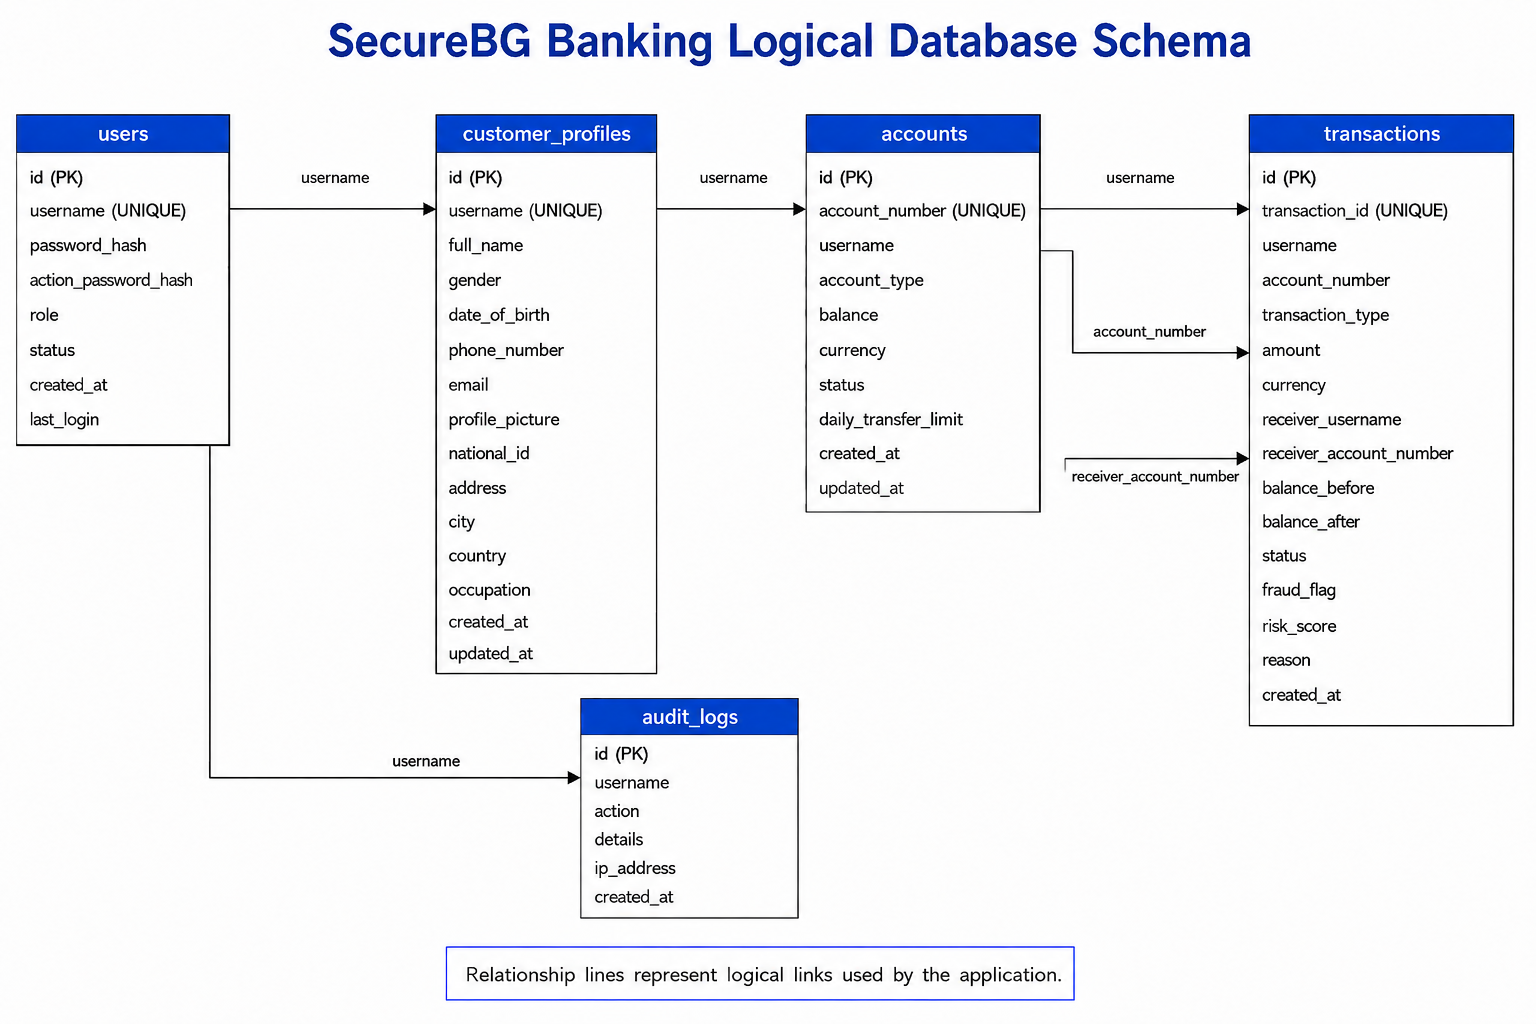
\includegraphics[width=\textwidth]{Banking-dabase-logical-schena.png}
    \caption{SecureBG banking logical database schema}
\end{figure}

\subsectionbreakguard
\subsection{Database Tables}

\begin{longtable}{|p{3.8cm}|p{10.2cm}|}
\hline
\textbf{Table} & \textbf{Purpose} \\
\hline
users & Stores login identity, password hash, action password hash, role, status, creation time, and last login time. \\
\hline
customer\_profiles & Stores personal customer profile fields such as full name, gender, date of birth, phone number, email, address, and occupation. \\
\hline
accounts & Stores account number, username, account type, balance, currency, status, and daily transfer limit. \\
\hline
transactions & Stores transaction ID, account number, transaction type, amount, receiver data, before and after balances, status, fraud flag, risk score, and reason. \\
\hline
audit\_logs & Stores system actions for user activity tracking. \\
\hline
\end{longtable}

\sectionbreakguard
\section{Main Workflows}

This section describes the main application workflows from the user's browser request to the backend RPC service and database operations. These workflows show how the distributed components cooperate to complete banking actions.

\subsectionbreakguard
\subsection{Registration and Login}

Registration starts when a new customer submits the registration form from the browser. Flask receives the form data, validates basic required fields, processes the optional profile picture upload, and sends the registration payload to the authentication RPC service. The authentication service normalizes the username, validates the submitted fields again, hashes both the login password and action password, creates the user record, creates the customer profile, creates the bank account, and writes a registration audit log.

Login starts when the customer submits a username and login password. Flask sends the credentials to the authentication RPC service. The authentication service loads the user record, verifies the submitted password with the stored hash, checks that the user account is active, updates the last login timestamp, writes a login audit log, and creates an encrypted Fernet ticket. Flask stores this ticket in the session. Later banking requests use the ticket instead of sending the login password again.

\subsectionbreakguard
\subsection{Dashboard Loading}

After login, the dashboard page gives the user a summary of account and risk information. Flask calls the banking service method \texttt{get\_dashboard\_summary}. The banking service validates the login ticket, loads profile information, loads account data, calculates the current risk score, counts total transactions, loads the latest transactions, and returns a combined dashboard response. Flask then renders the dashboard page with the balance, account number, account status, risk score, recent transactions, and profile picture.

\subsectionbreakguard
\subsection{Deposit}

Deposit is the simplest money workflow because it requires only a valid login ticket and a positive amount. Flask validates that the amount is greater than zero and calls \texttt{deposit}. The banking service validates the ticket, loads the account, checks account status, calculates the new balance, runs the fraud detection rules, updates the account balance, records the deposit transaction, and writes an audit log. The service returns the new balance and risk result to Flask.

\subsectionbreakguard
\subsection{Withdraw}

Withdraw is more sensitive than deposit because money leaves the account. The user must provide the amount and action password. Flask checks that the amount is valid and that an action password was submitted. The banking service validates the login ticket, checks the action password against the stored action password hash, verifies that the account has enough balance, calculates the new balance, runs fraud detection, updates the balance, records the withdrawal transaction, and writes an audit log. If the action password is incorrect or the balance is insufficient, the service records a failed transaction and returns an error message.

\subsectionbreakguard
\subsection{Transfer}

Transfer requires cooperation between the sender account and receiver account. The user submits the receiver username, amount, and action password. Flask validates the basic fields and prevents self-transfer before calling the banking service. The banking service validates the sender ticket, normalizes the receiver username, verifies the action password, loads sender and receiver accounts, checks receiver account status, checks sender balance, calculates sender and receiver balances, and runs fraud detection for the sender. After validation, the service updates both account balances, saves a \texttt{TRANSFER\_OUT} record for the sender, saves a \texttt{TRANSFER\_IN} record for the receiver, and writes audit logs for both accounts.

\subsectionbreakguard
\subsection{Transaction History}

The transaction history page shows all transaction records for the logged-in user. Flask calls \texttt{view\_transaction\_history} with the login ticket. The banking service validates the ticket, loads the user transaction records from SQLite, and returns them to Flask. The page displays transaction type, amount, receiver information, balances before and after, status, risk score, fraud flag, reason, and timestamp.

\subsectionbreakguard
\subsection{Fraud Detection}

Fraud detection is rule-based. It calculates a risk score and marks transactions as suspicious when the score reaches the configured threshold. The rules include:

\begin{longtable}{|p{1.2cm}|p{12.8cm}|}
\hline
\textbf{No.} & \textbf{Fraud rule} \\
\hline
1 & Account status problems. \\
\hline
2 & Large transaction amount. \\
\hline
3 & Amount much higher than the user's average transaction amount. \\
\hline
4 & Many transactions in a short time window. \\
\hline
5 & Large balance drop after withdraw or transfer. \\
\hline
6 & Transfers to many different receivers quickly. \\
\hline
7 & Transfer amount exceeding the daily transfer limit. \\
\hline
\end{longtable}

The fraud report page calls \texttt{detect\_fraud}. The banking service validates the ticket and asks the fraud detection module to summarize the user's suspicious transactions. The report contains a fraud flag, total risk score, reason list, and suspicious transaction records. The user can also trust suspicious results through \texttt{trust\_fraud\_report}, which resets the fraud flag and risk score for suspicious transactions after user review.

\subsectionbreakguard
\subsection{Profile Update}

The profile workflow allows the user to view and update editable customer information. Flask first calls \texttt{get\_user\_profile} to load the current profile and account details. When the user submits profile changes, Flask validates required fields such as full name, phone number, and email. If a new profile picture is uploaded, Flask validates the image extension, resizes the image, and stores it in the upload folder. The updated profile data is then sent to \texttt{update\_user\_profile}. The banking service validates the ticket and updates the customer profile in SQLite.

\sectionbreakguard
\section{Implementation Details}

\subsectionbreakguard
\subsection{Encrypted Login Ticket}

After successful login, the authentication service creates a Fernet encrypted ticket containing the username, issue time, and expiry time. The banking service decrypts and validates this ticket before allowing banking operations. This approach separates authentication from banking operations while still allowing the banking service to identify the current user.

\subsectionbreakguard
\subsection{Action Password}

The application uses a second password called the action password. It is required for sensitive money-moving operations such as withdraw and transfer. This gives stronger protection than using only the login password.

\subsectionbreakguard
\subsection{Logging}

The project includes structured logging for the web app, authentication RPC service, banking RPC service, fraud detection module, and database layer. The logs help demonstrate how data moves across the distributed services during registration, login, deposit, withdraw, transfer, and fraud detection.

\sectionbreakguard
\section{Result Screenshots}

\begin{figure}[H]
    \centering
    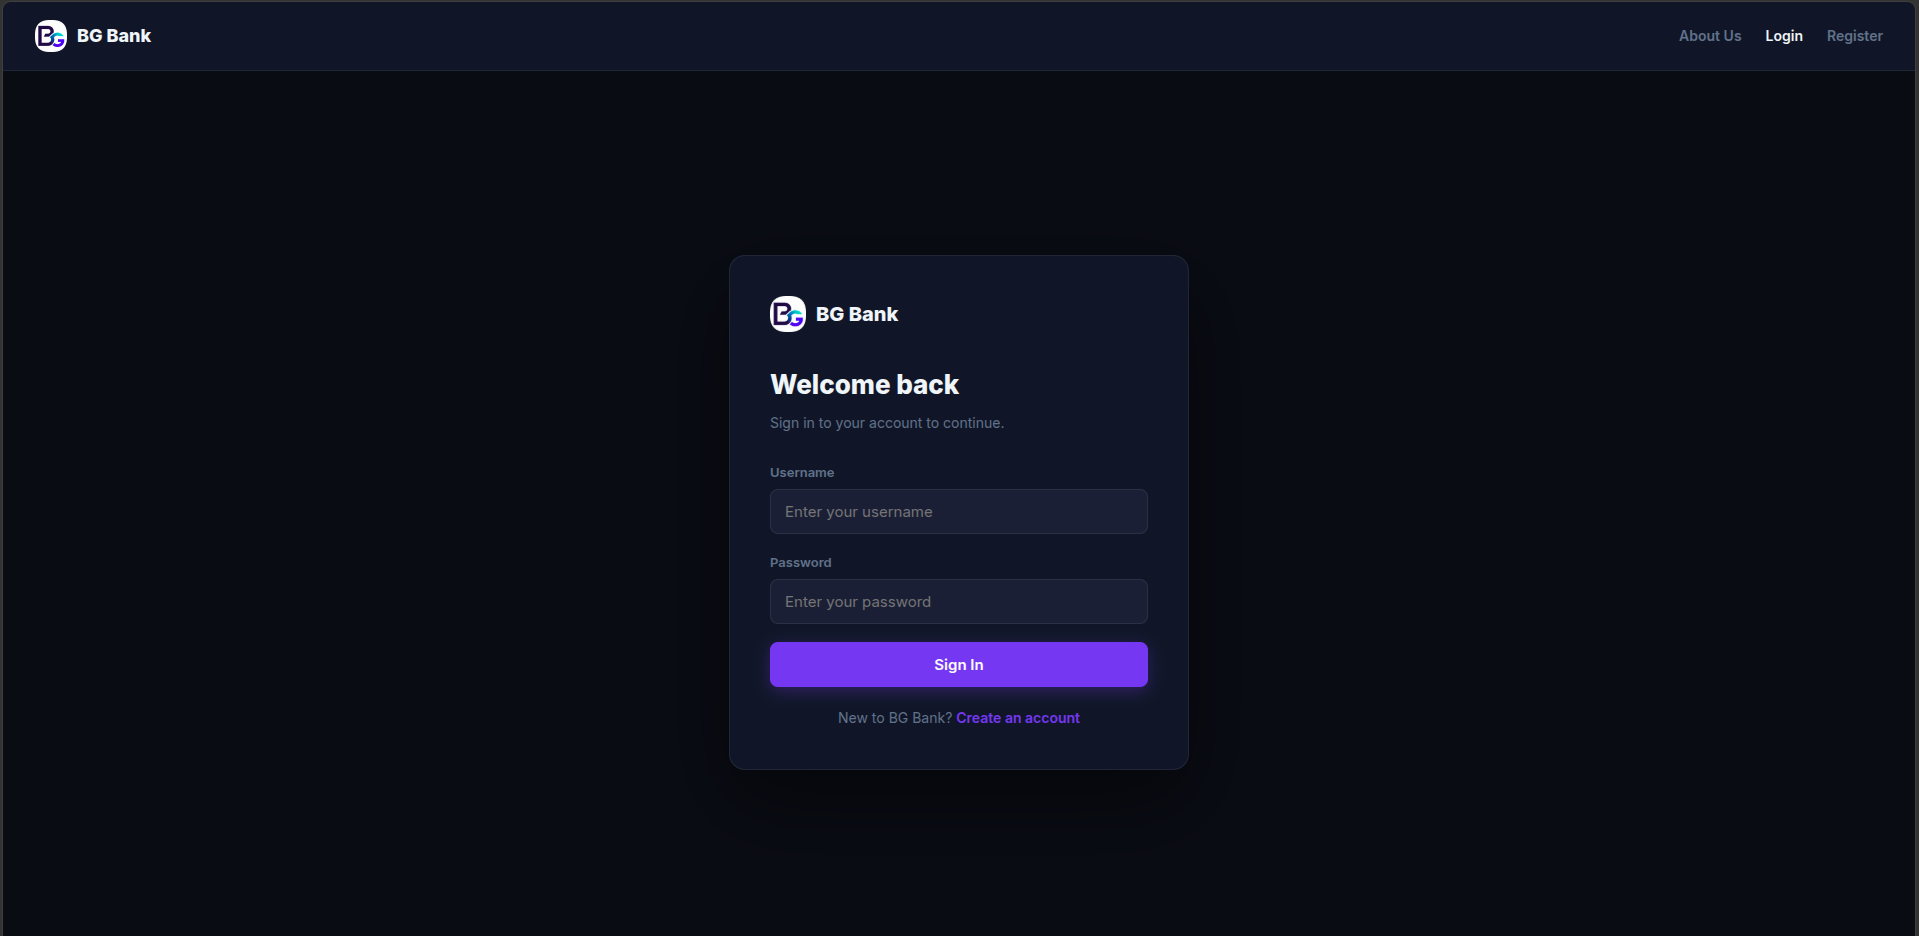
\includegraphics[width=0.95\textwidth]{login-web-view.png}
    \caption{Login page}
\end{figure}

\begin{figure}[H]
    \centering
    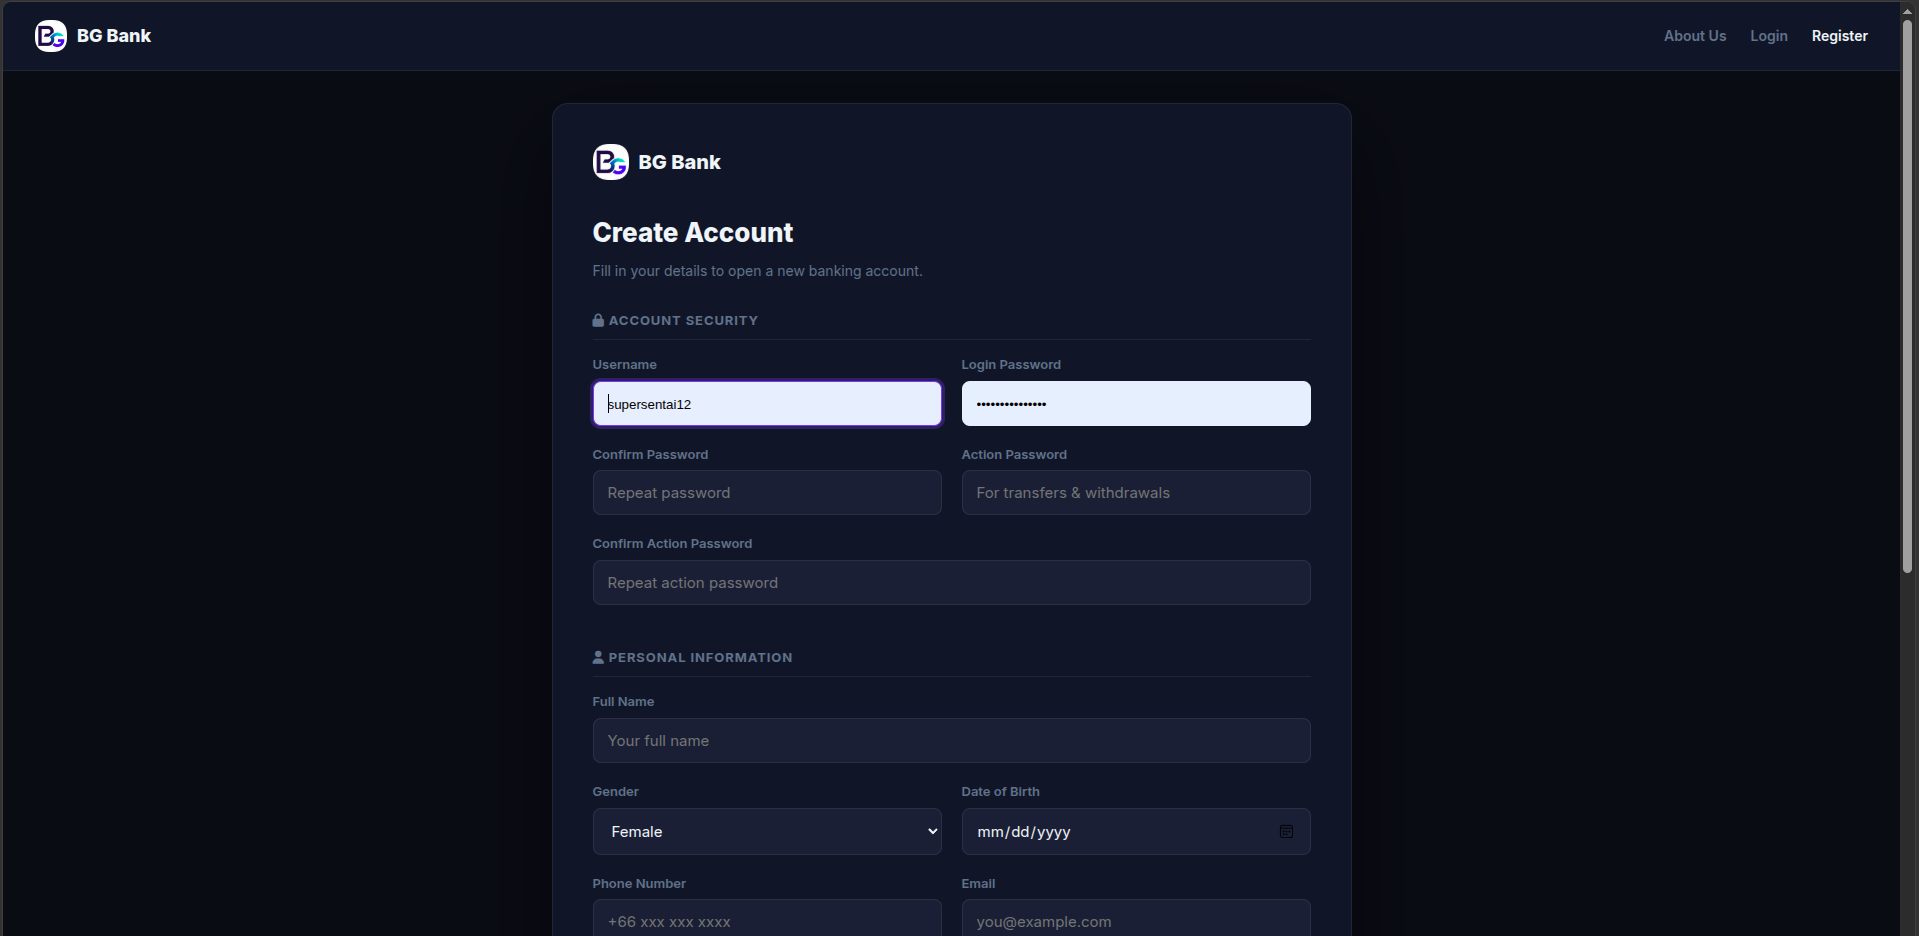
\includegraphics[width=0.95\textwidth]{register-web-view.png}
    \caption{Registration page}
\end{figure}

\begin{figure}[H]
    \centering
    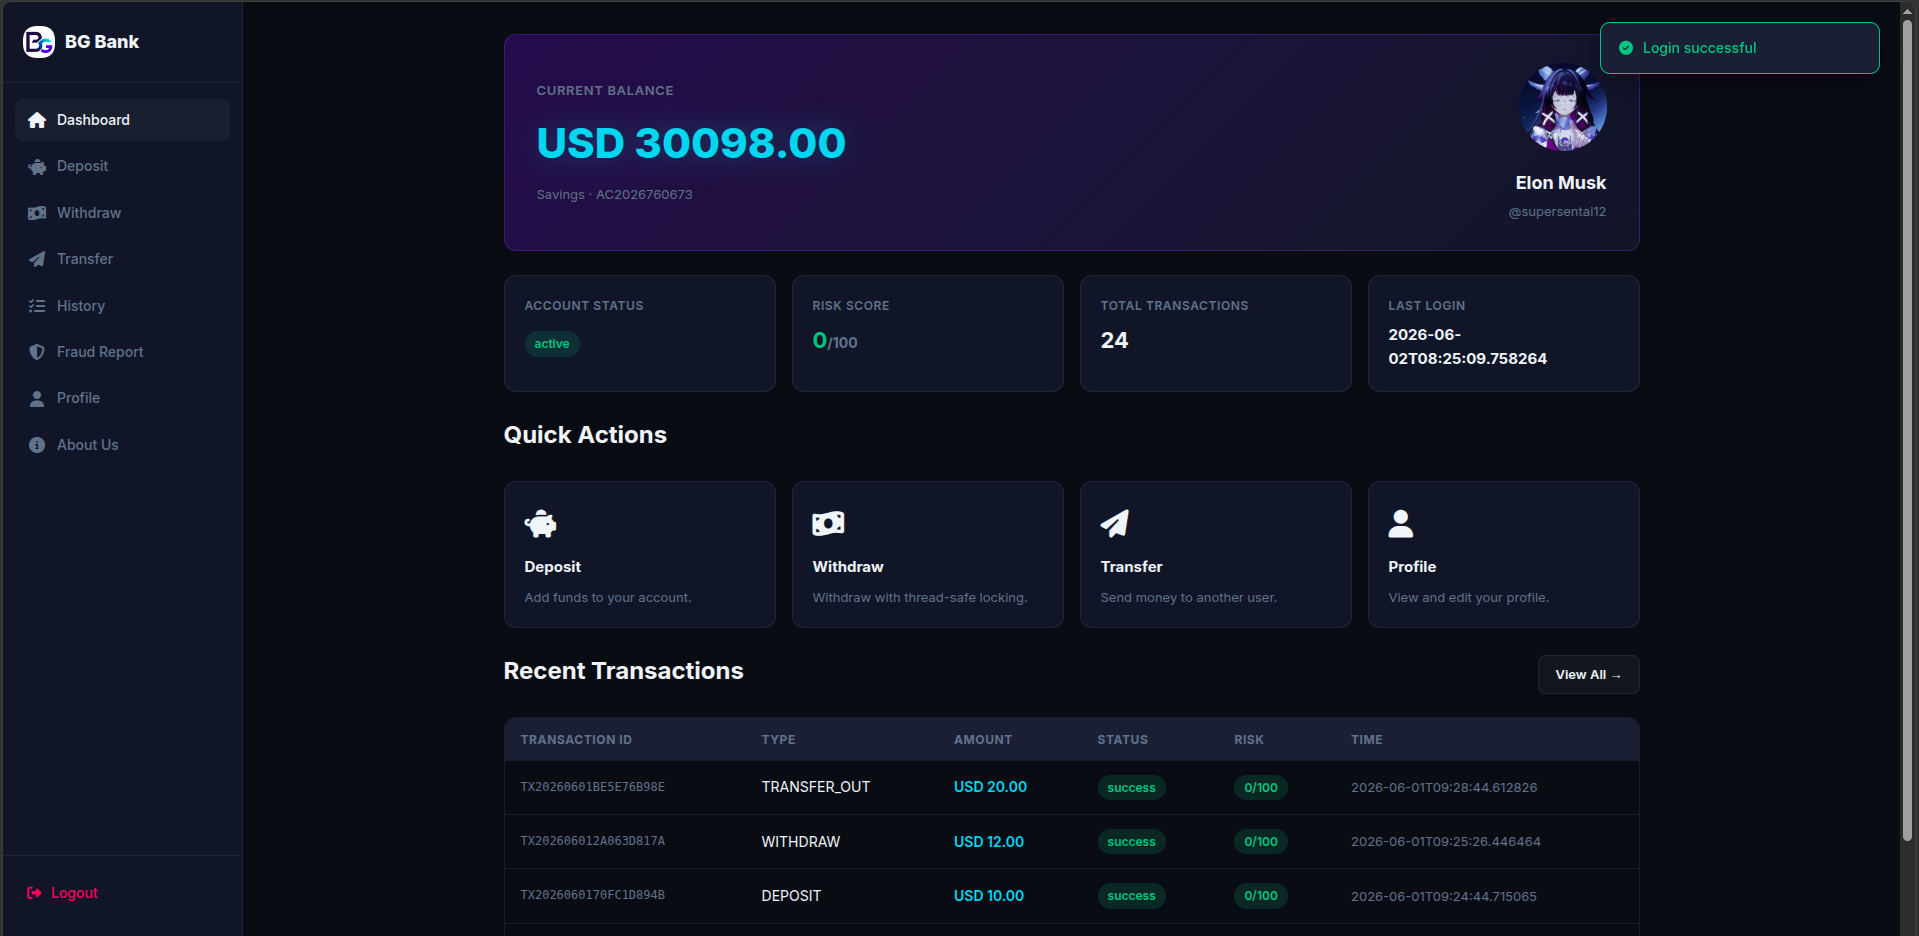
\includegraphics[width=0.95\textwidth]{dashboard-web-view.png}
    \caption{Dashboard page}
\end{figure}

\begin{figure}[H]
    \centering
    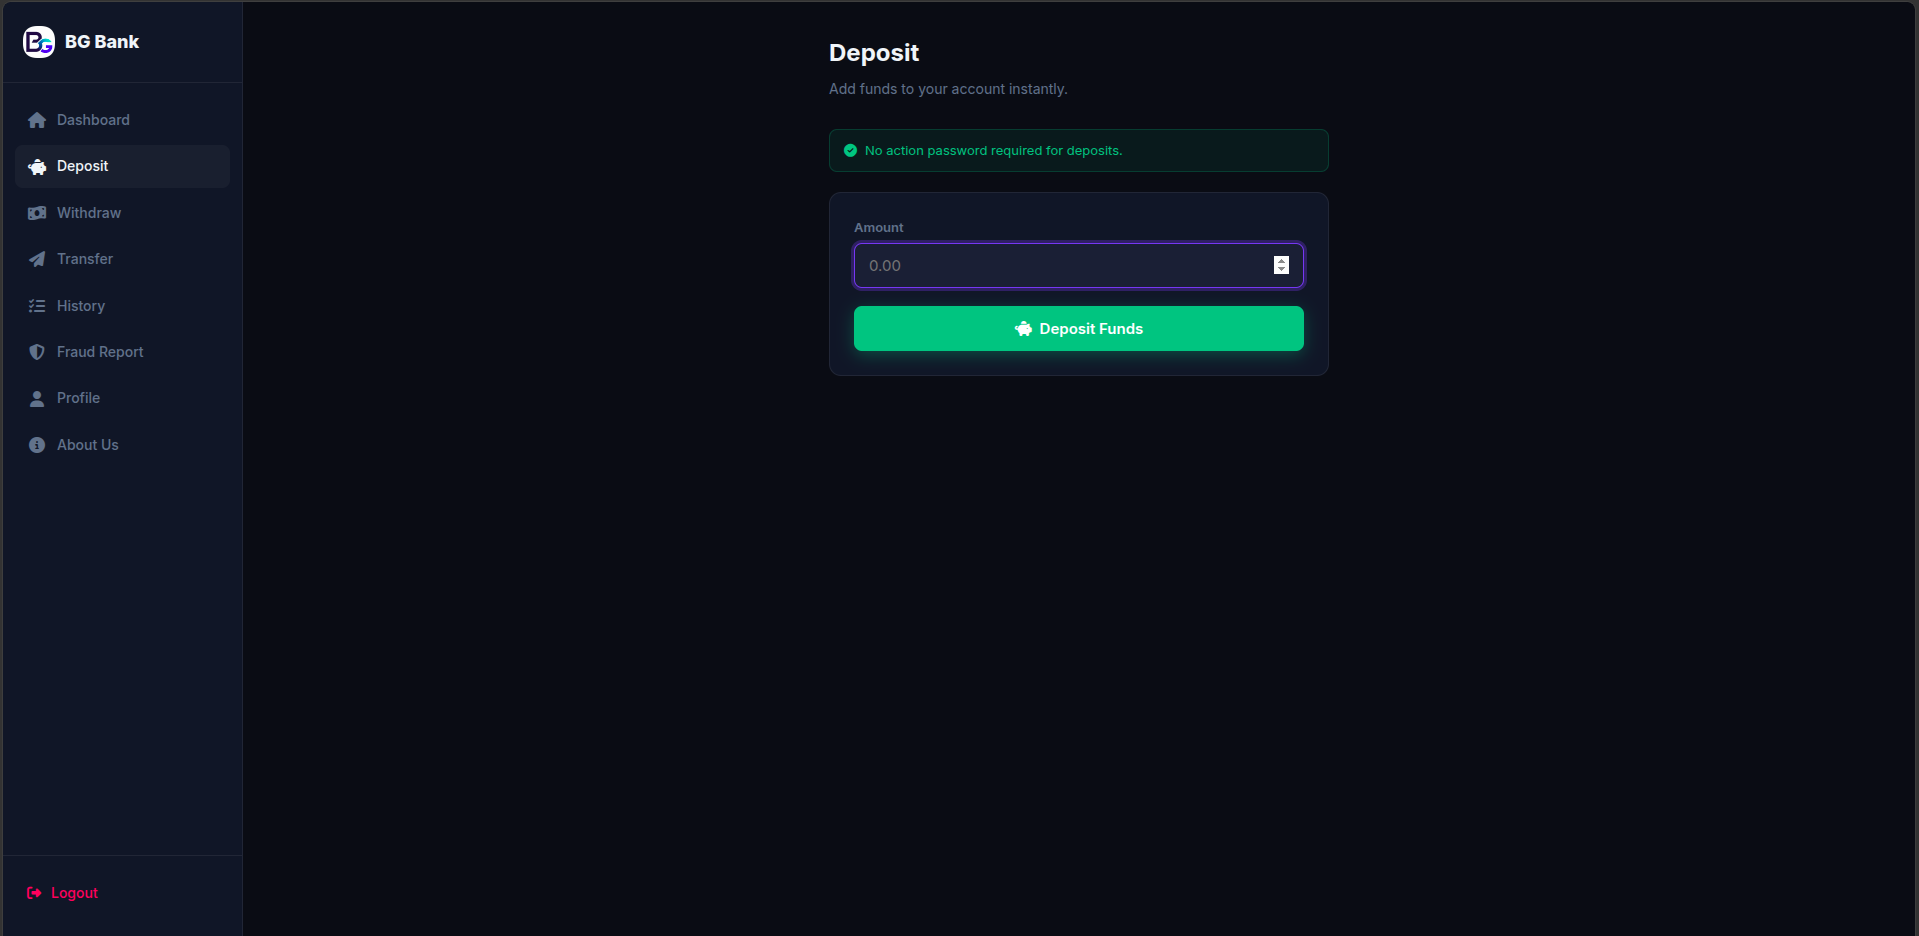
\includegraphics[width=0.95\textwidth]{deposit-web-view.png}
    \caption{Deposit page}
\end{figure}

\begin{figure}[H]
    \centering
    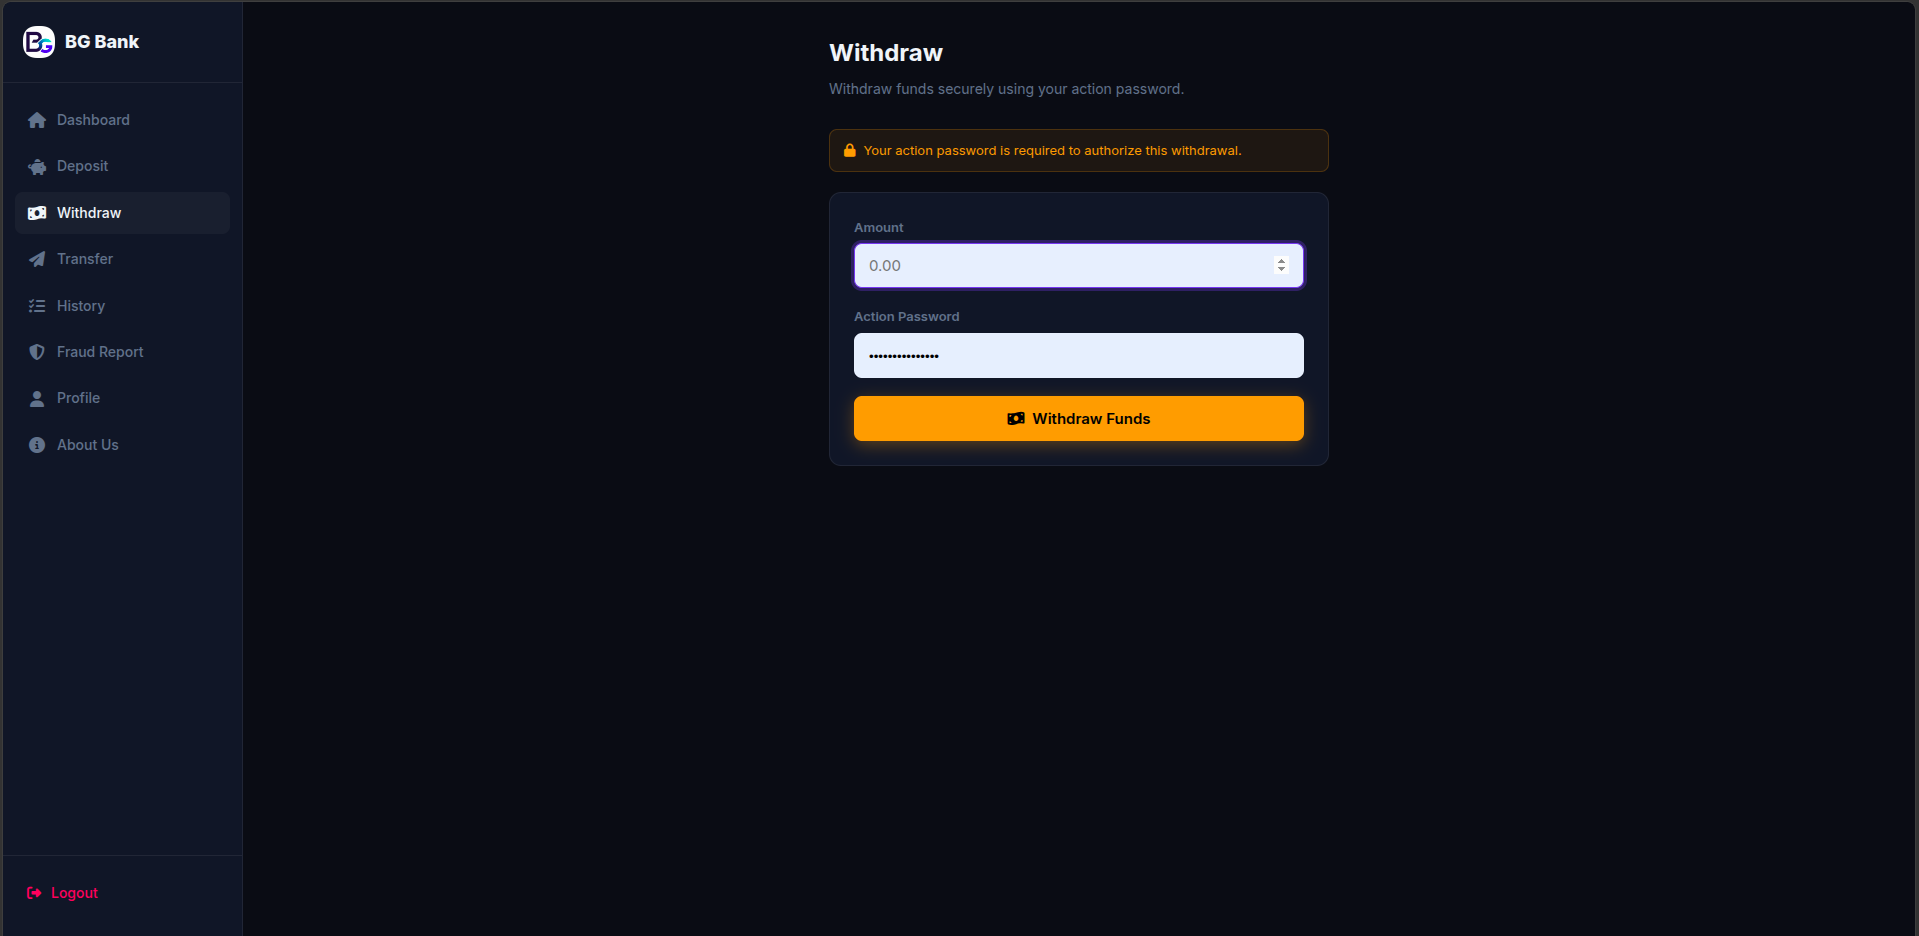
\includegraphics[width=0.95\textwidth]{withdraw-view.png}
    \caption{Withdraw page}
\end{figure}

\begin{figure}[H]
    \centering
    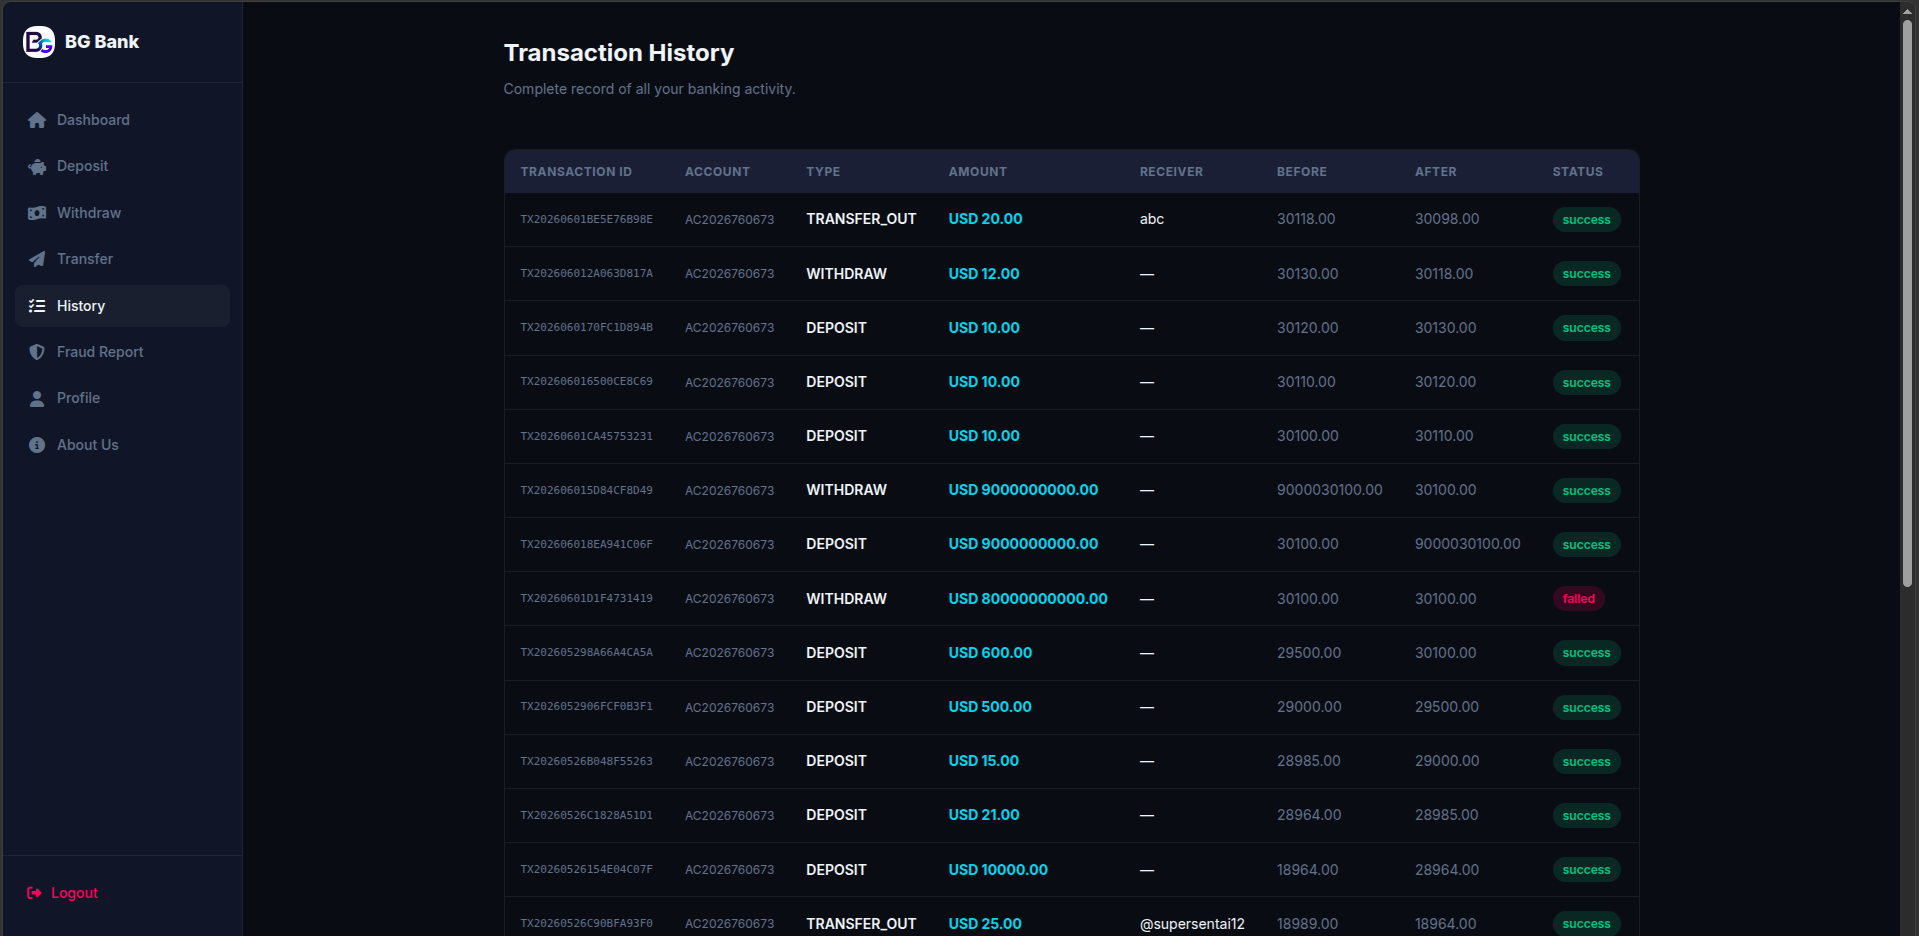
\includegraphics[width=0.95\textwidth]{history-web-view.png}
    \caption{Transaction history page}
\end{figure}

\begin{figure}[H]
    \centering
    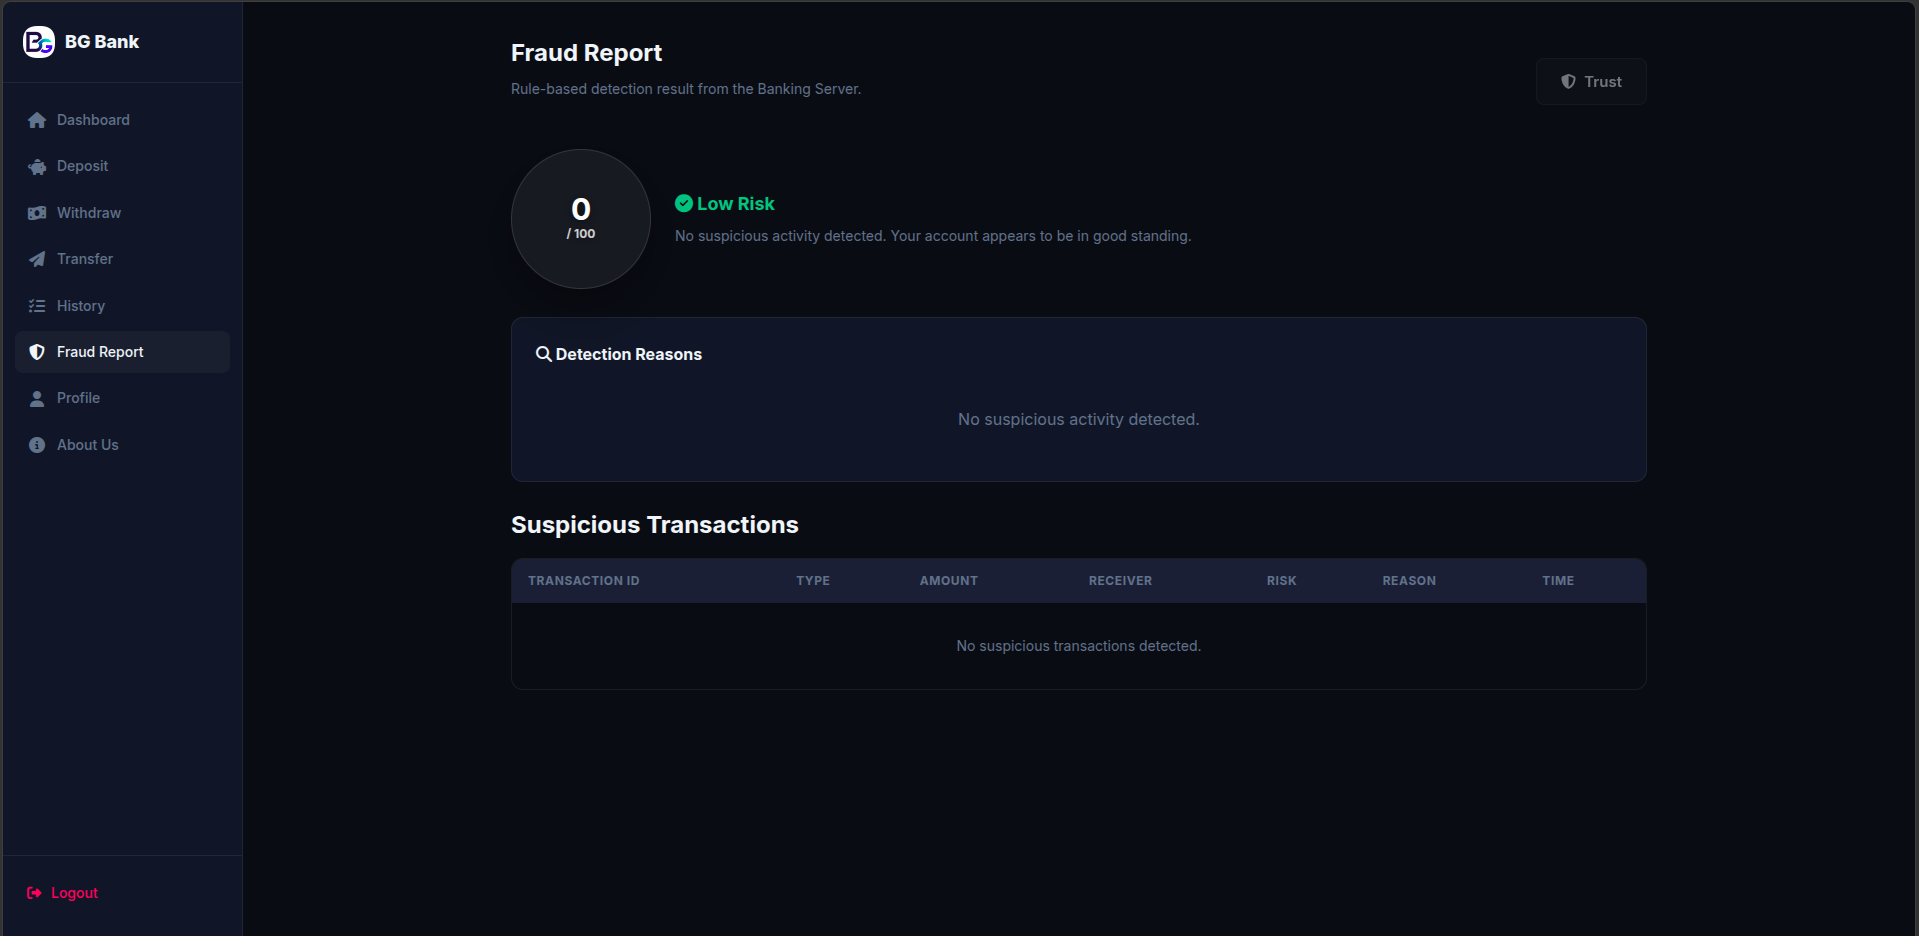
\includegraphics[width=0.95\textwidth]{fraid-report-web-view.png}
    \caption{Fraud report page}
\end{figure}

\begin{figure}[H]
    \centering
    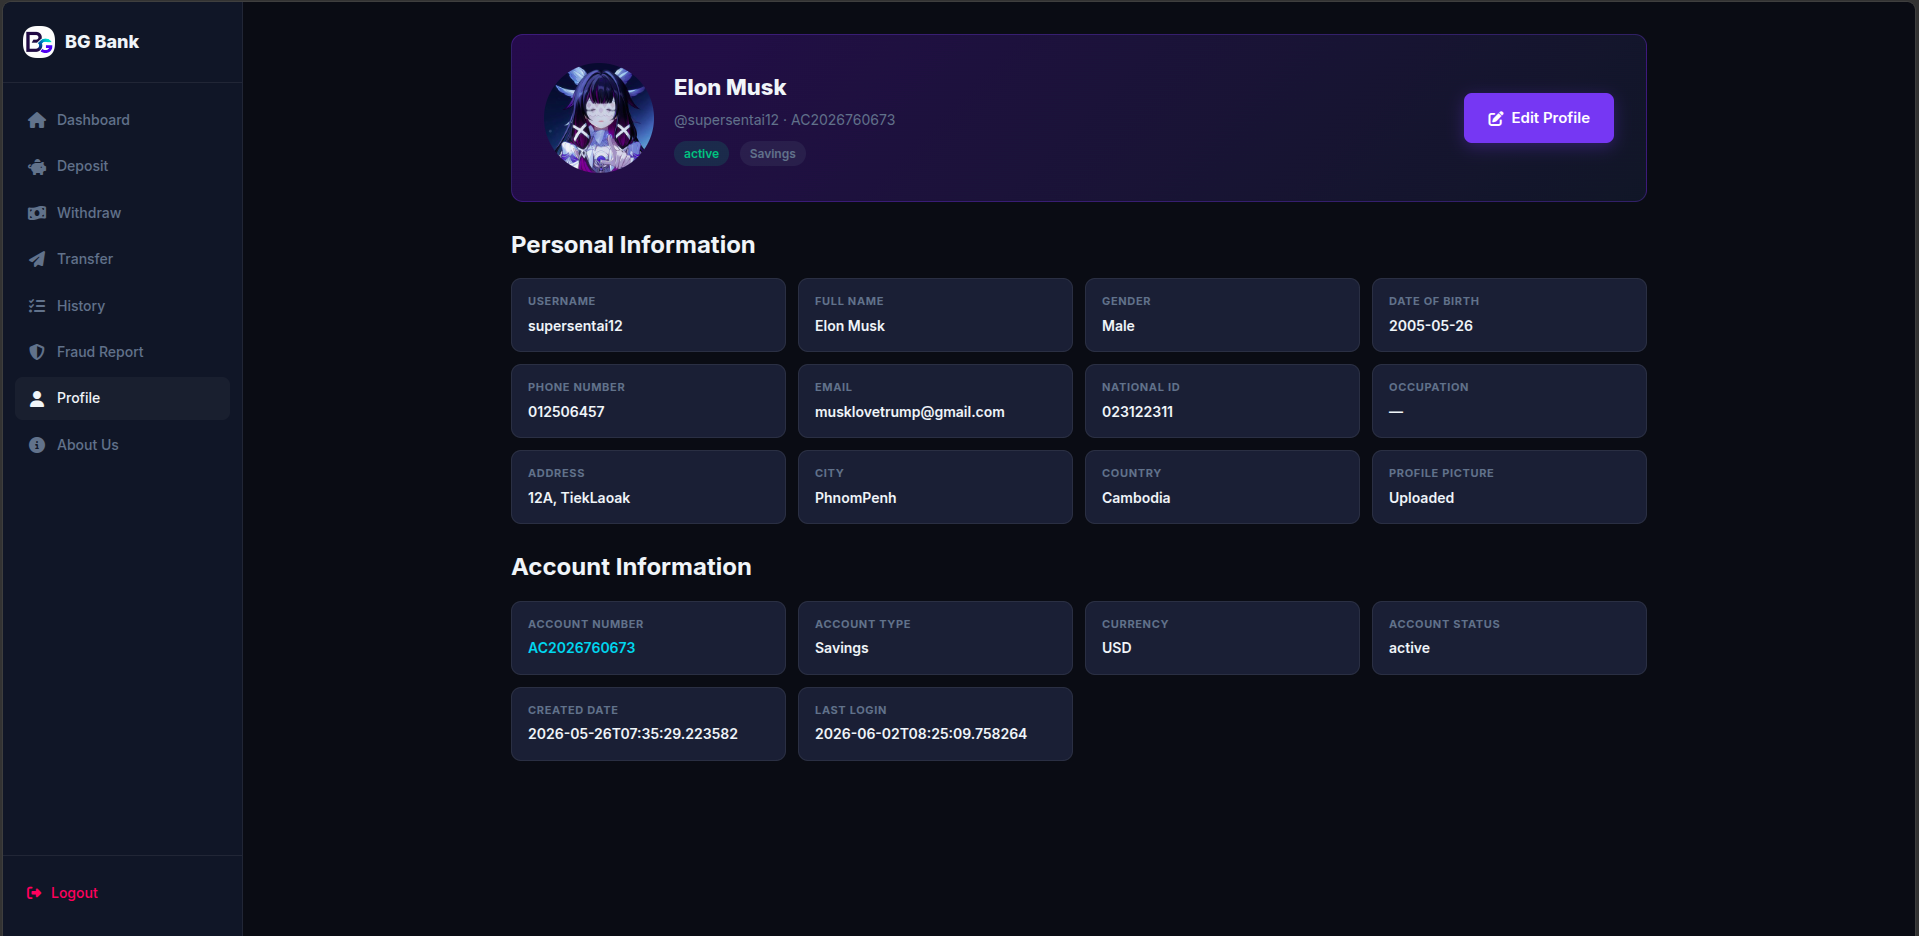
\includegraphics[width=0.95\textwidth]{profile-web-view.png}
    \caption{Profile page}
\end{figure}

\begin{figure}[H]
    \centering
    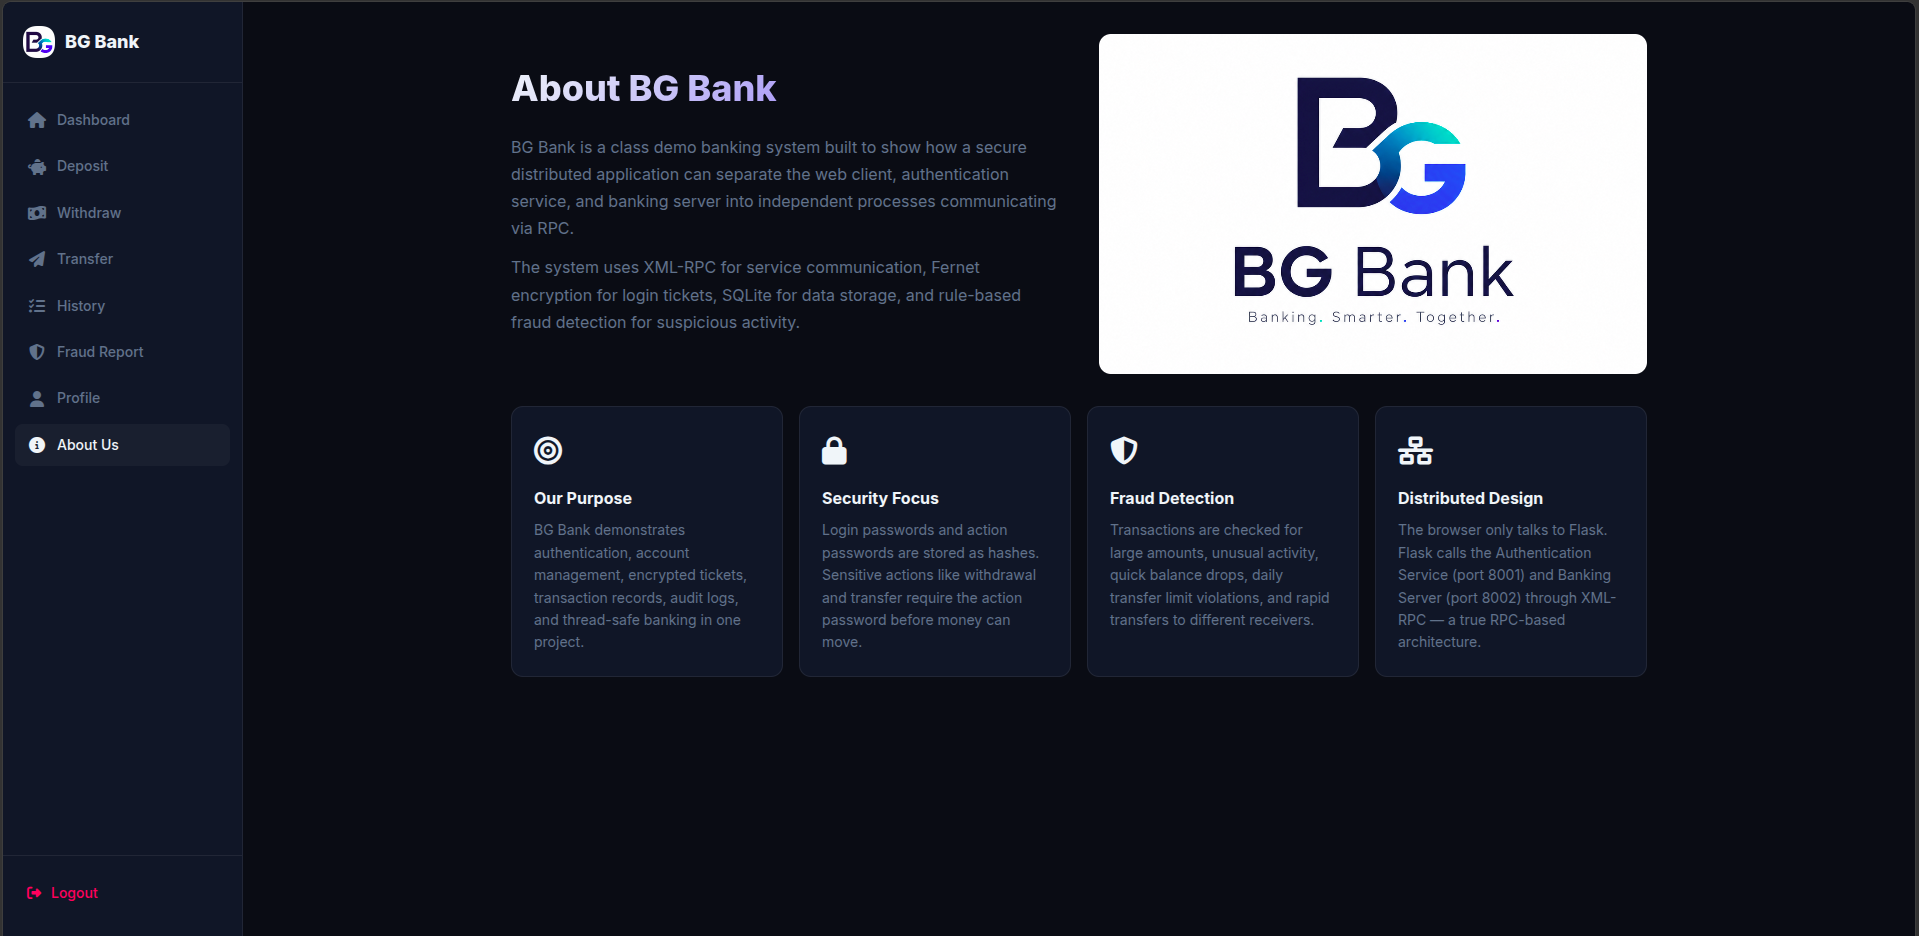
\includegraphics[width=0.95\textwidth]{aboutus-web-view.png}
    \caption{About page}
\end{figure}

\begin{figure}[H]
    \centering
    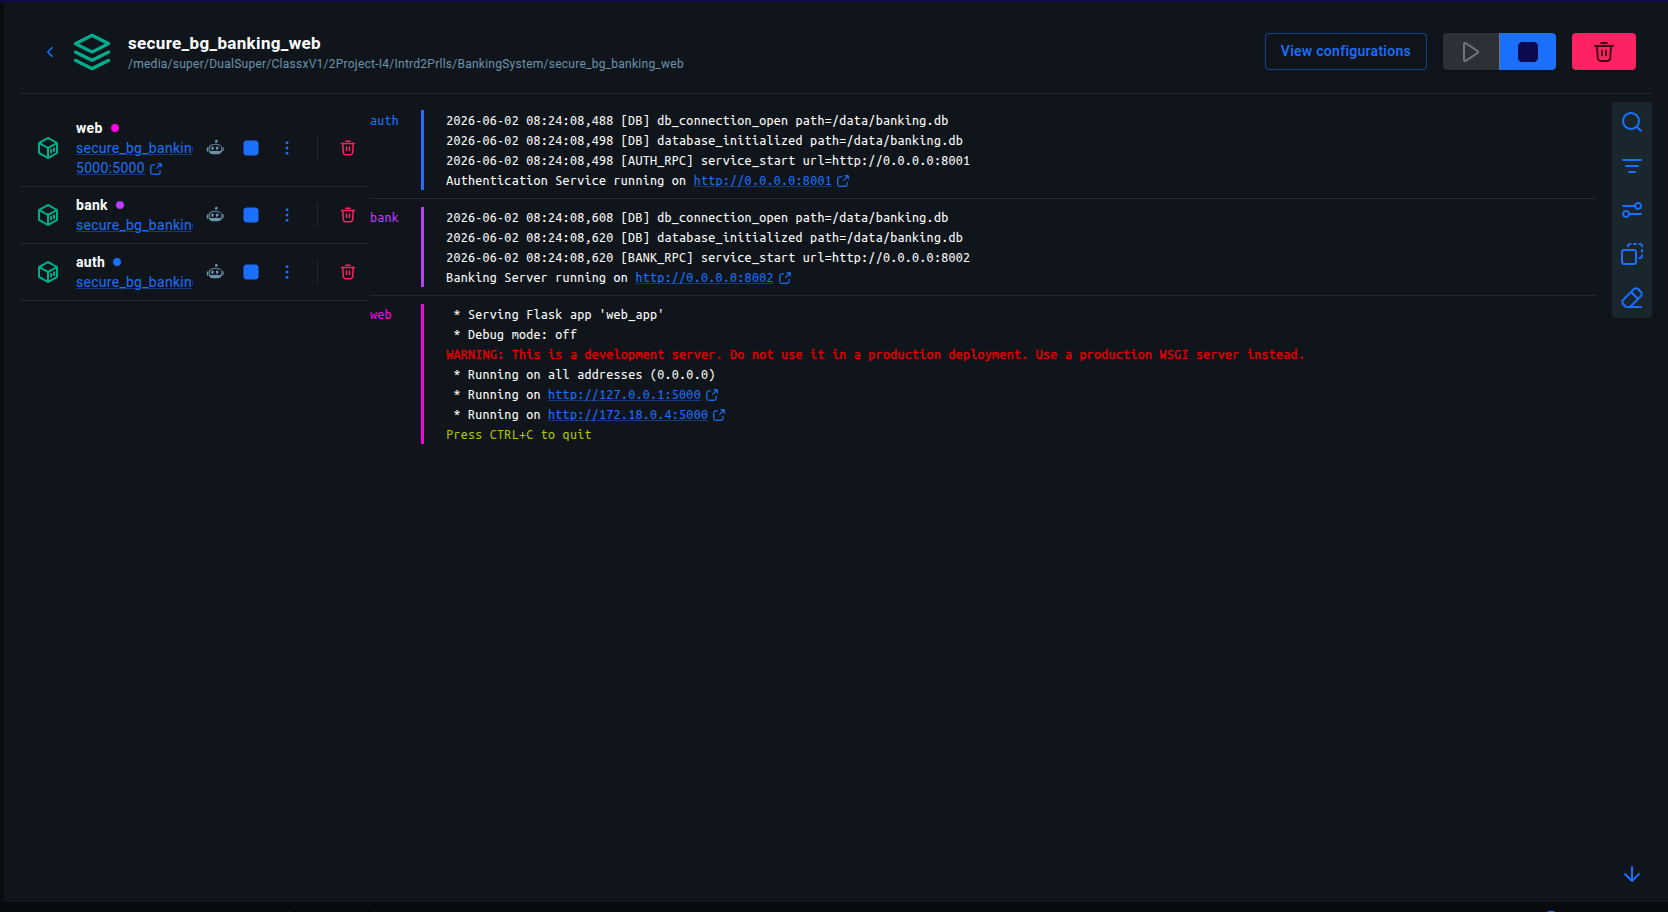
\includegraphics[width=0.95\textwidth]{docker-hosting-view.png}
    \caption{Docker hosting view}
\end{figure}

\begin{figure}[H]
    \centering
    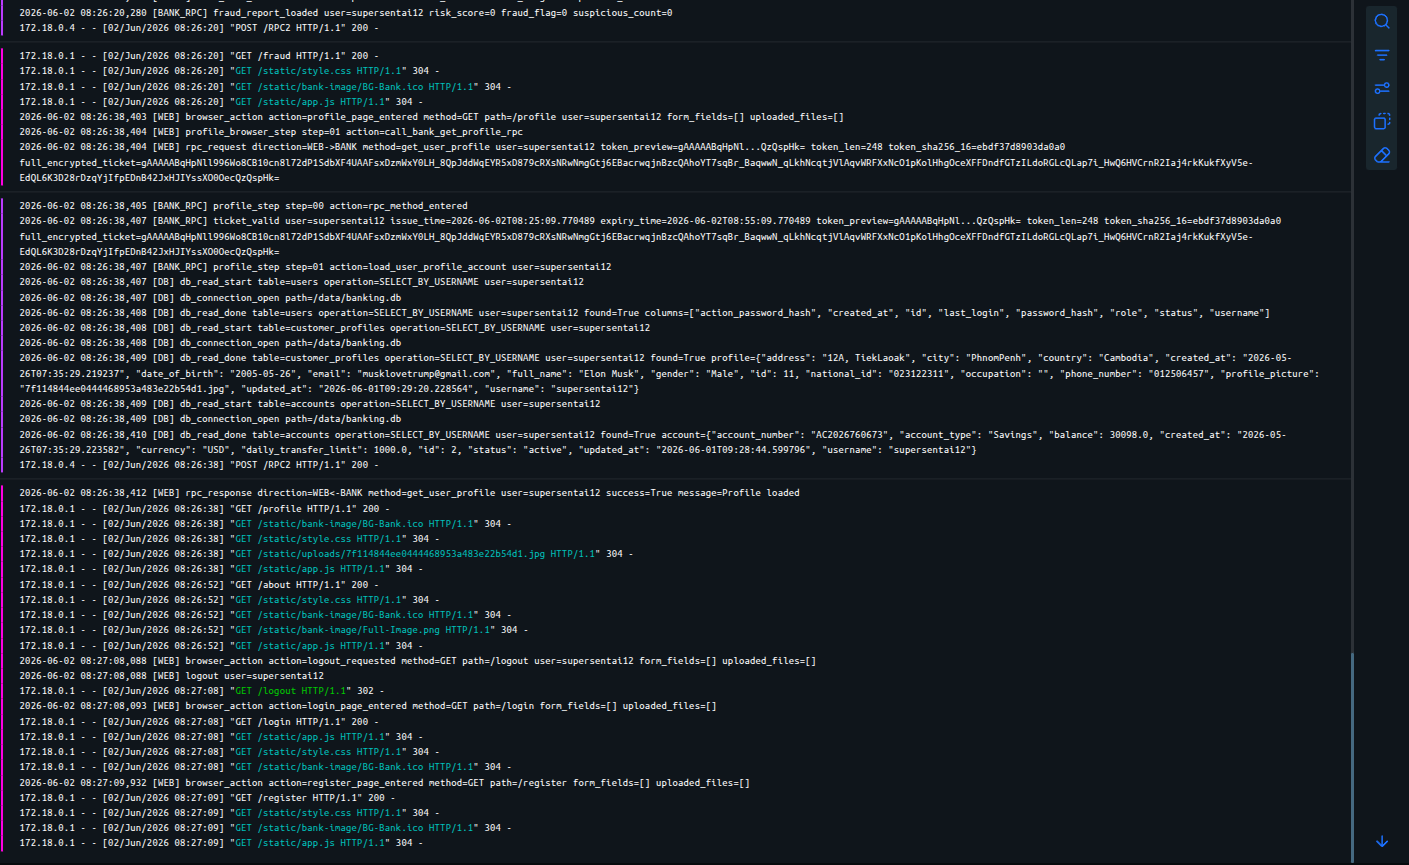
\includegraphics[width=0.95\textwidth]{docker-logs-process-views.png}
    \caption{Docker logs and service process view}
\end{figure}

\sectionbreakguard
\section{Security Discussion}

The project includes several security mechanisms that are appropriate for a demonstration banking system. These mechanisms protect authentication, restrict sensitive operations, track suspicious behavior, and record important user actions.

\subsectionbreakguard
\subsection{Password Storage}

The system does not store plain text passwords. Both the login password and action password are stored as hashes. The login password is used only for authentication, while the action password is used to approve sensitive money-moving operations. This separation reduces the risk that a stolen login session alone can immediately perform withdrawals or transfers.

\subsectionbreakguard
\subsection{Encrypted Login Ticket}

After a successful login, the authentication service creates a Fernet encrypted ticket. The ticket contains the username, issue time, and expiry time. Flask stores the ticket in the user session and sends it to the banking service when performing account operations. The banking service decrypts and validates the ticket before processing the request. If the ticket is invalid or expired, the service rejects the operation.

This ticket-based design supports service separation. The authentication service proves the user's identity once during login, and the banking service later validates the ticket without receiving the login password again.

\subsectionbreakguard
\subsection{Action Password Protection}

Withdraw and transfer require the action password. The banking service checks the submitted action password against the stored action password hash before allowing money to leave the account. Deposit does not require the action password because it only increases the user's balance. This design gives the system two levels of protection: login authentication for session access and action password verification for sensitive transactions.

\subsectionbreakguard
\subsection{Fraud Monitoring}

The fraud detection module records suspicious transaction behavior using a rule-based score. The rules are simple but useful for demonstration because they show how transaction monitoring can be added to a distributed banking workflow. Suspicious transactions keep their risk score and reason in the database, which allows the dashboard and fraud report page to show the current risk status to the user.

\subsectionbreakguard
\subsection{Audit Logging}

Audit logs record important actions such as registration, login, deposit, withdraw, transfer, profile update, and fraud report trust actions. These logs help explain system behavior during demonstrations and can support later review of user activity. In a production system, audit logs should be protected from modification and should avoid exposing sensitive secrets.

\subsectionbreakguard
\subsection{Security Limitations}

The project is designed for learning and demonstration, so it still has limitations that should be addressed before production use:

\begin{longtable}{|p{1.2cm}|p{12.8cm}|}
\hline
\textbf{No.} & \textbf{Security limitation} \\
\hline
1 & Sensitive research logging should be disabled in production because logs can expose password hashes, password fingerprints, encrypted tickets, registration payloads, profile data, balances, and transaction details. \\
\hline
2 & Web forms should include CSRF protection to prevent forged form submissions from another website. \\
\hline
3 & XML-RPC traffic should run over HTTPS or a protected internal network so tickets and transaction data are not exposed in transit. \\
\hline
4 & Login attempts should have rate limiting or account lockout rules to reduce brute-force password attacks. \\
\hline
5 & Uploaded profile images should be scanned and served with strict file handling rules. \\
\hline
6 & Session cookies should use secure cookie settings when deployed with HTTPS. \\
\hline
\end{longtable}

\sectionbreakguard
\section{Limitations and Future Improvements}

The current project demonstrates the main concepts of RPC communication, service separation, ticket authentication, and banking workflows. However, several improvements are needed to make the design stronger and closer to a production banking system.

\subsectionbreakguard
\subsection{Atomic Database Transactions}

Deposit, withdraw, transfer, and registration perform several database operations. For example, transfer updates the sender balance, updates the receiver balance, creates two transaction records, and writes audit logs. These operations should be wrapped in database transactions so that either all changes succeed together or all changes are rolled back together. This would prevent inconsistent balances or incomplete records after an error.

\subsectionbreakguard
\subsection{Safer Money Representation}

The current implementation uses floating point values for money. Floating point arithmetic can create rounding errors. A safer design would store money as integer cents or use Python \texttt{Decimal}. This would make balance calculations more reliable.

\subsectionbreakguard
\subsection{Database Constraints}

The database uses logical relationships through fields such as username and account number, but it does not enforce all relationships with formal foreign key constraints. Future versions should add stronger constraints for users, profiles, accounts, transactions, and audit logs. This would reduce invalid references and improve data integrity.

\subsectionbreakguard
\subsection{Improved Authentication Controls}

The system could be improved with password strength rules, password reset workflow, login rate limiting, account lockout after repeated failed attempts, and optional multi-factor authentication. These controls would make authentication more realistic for a banking application.

\subsectionbreakguard
\subsection{Improved Fraud Detection}

The current fraud detection rules are fixed thresholds. Future work could include configurable thresholds, admin review tools, account freezing, notification services, and machine-learning based risk scoring. The fraud report could also separate low, medium, and high severity transactions.

\subsectionbreakguard
\subsection{Testing and Reliability}

Automated tests should be added for registration, login, ticket expiry, deposit, withdraw, transfer, fraud detection, profile update, and failed transaction cases. Integration tests should verify that Flask, the authentication service, banking service, and database work correctly together. This would make future changes safer.

\subsectionbreakguard
\subsection{Deployment Improvements}

The Docker setup is useful for demonstration. A production-style deployment should use HTTPS, secure environment variables, separated secrets, restricted database access, centralized logging, and backup procedures. Service health checks and monitoring would also improve reliability.

\sectionbreakguard
\section{Conclusion}

BG Bank demonstrates a distributed banking application using Flask and XML-RPC services. The project separates web presentation, authentication, banking logic, fraud detection, and database storage into clear components. It shows how encrypted tickets and action passwords can protect banking operations, and how rule-based fraud detection can help identify suspicious transactions. The application is suitable for demonstrating RPC communication, service coordination, shared database access, and security concerns in distributed systems.

\end{document}
